\clearpage
\section{Visualizing Matrix Arithmetic in 2D}\label{sec:geom_1}



\asyouread{
\item	T/F: Two vectors with the same length and direction are equal even if they start from different places.
%\item	T/F: Adding two vectors together forms a parallelogram.
\item 	One can visualize vector addition using what law?
\item	T/F: Multiplying a vector by 2 doubles its length.
\item	What do mathematicians do?
\item	T/F: Multiplying a vector by a  matrix always changes its length and direction.
}

When we first learned about adding numbers together, it was useful to picture a number line: $2+3=5$ could be pictured by starting at 0, going out 2 tick marks, then another 3, and then realizing that we moved 5 tick marks from 0. Similar visualizations helped us understand what $2-3$ meant and what $2\times 3$ meant.


We now investigate a way to picture matrix arithmetic -- in particular, operations involving column vectors. This not only will help us better understand the arithmetic operations, it will open the door to a great wealth of interesting study. Visualizing matrix arithmetic has a wide variety of applications, the most common being computer graphics. While we often think of these graphics in terms of video games, there are numerous other important applications. For example, chemists and biologists often use computer models to ``visualize'' complex molecules to ``see'' how they interact with other molecules.%This section contains many figures. In order to reduce the clutter of the graphs, we will use the convention that each tick mark represents one unit, unless specified otherwise.}\\ %Also, in some cases the placement of the figures is a bit odd -- they don't appear immediately near the statements that refer to them. Therefore take care to look at the captions of the Figures to see what example they refer to.}\\


We will start with vectors in two dimensions (2D) -- that is, vectors with only two entries. We assume the reader is familiar with the Cartesian plane, that is, plotting points and graphing functions on ``the $x$--$y$ plane.'' We graph vectors in a manner very similar to plotting points. Given the vector $$\vx = \bmx{c}1\\2\emx,$$ we draw \vx\ by drawing an arrow whose tip is 1 unit to the right and 2 units up from its origin.\footnote{To help reduce clutter, in all figures each tick mark represents one unit.} 

%\begin{myfigure}%[h!]
%\begin{center}
%\begin{tikzpicture}[scale=.75]%[x={(.5cm,0)},y={(0,.5cm)}]
%\draw (-3,0)--(3,0);
%\draw (0,-3)--(0,3);
%\foreach \x in {-2,...,2}
% {\draw  (\x,-.1)--(\x,.1);
%  \draw  (-.1,\x)--(.1,\x);
% };
%\node[below] at (1,-0.1) {1};
%\node[left] at (0,1) {1};
%\draw [->,thick,>=latex] (0,0)--(1,2);
%\draw [->,thick,>=latex] (-2,-2)--(-1,0);
%\draw [->,thick,>=latex] (1,-1)--(2,1);
%\end{tikzpicture}
%\end{center}
%\mycaption{Various drawings of $\protect\vx$}
%\label{fig:draw_vectors}
%\end{myfigure}%

\enlargethispage{2\baselineskip}

\begin{myfigure}
\begin{center}
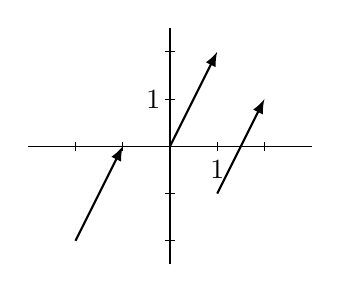
\begin{tikzpicture}[scale=.6]%[x={(.5cm,0)},y={(0,.5cm)}]
\draw (-3,0)--(3,0);
\draw (0,-2.5)--(0,2.5);
\foreach \x in {-2,...,2}
 {\draw  (\x,-.1)--(\x,.1);
  \draw  (-.1,\x)--(.1,\x);
 };
\node[below] at (1,-0.1) {1};
\node[left] at (0,1) {1};
\draw [->,thick,>=latex] (0,0)--(1,2);
\draw [->,thick,>=latex] (-2,-2)--(-1,0);
\draw [->,thick,>=latex] (1,-1)--(2,1);
\end{tikzpicture}
\end{center}
\mycaption{Various drawings of $\protect\vx$}
\label{fig:draw_vectors}
\end{myfigure}

When drawing vectors, we do not specify where you start drawing; all we specify is where the tip lies based on where we started. Figure \ref{fig:draw_vectors} shows vector \vx\ drawn 3 ways. In some ways, the ``most common'' way to draw a vector has the arrow start at the origin,%\footnote{the ``origin'' of the arrow is at the origin}
 but this is by no means the only way of drawing the vector.

Let's practice this concept by drawing various vectors from given starting points.\\

\example{ex_draw_vectors_1}{Let $$\vx = \bmx{c}1\\-1\emx \quad \vy = \bmx{c} 2\\3\emx \quad \text{ and } \quad \vz = \bmx{c} -3\\2\emx.$$
Draw \vx\ starting from the point $(0,-1)$; draw \vy\ starting from the point $(-1,-1)$, and draw \vz\ starting from the point $(2,-1)$.}
{To draw \vx, start at the point $(0,-1)$ as directed, then move to the right one unit and down one unit and draw the tip. Thus the arrow ``points'' from $(0,-1)$ to $(1,-2)$.

To draw \vy, we are told to start and the point $(-1,-1)$. We draw the tip by moving to the right 2 units and up 3 units; hence \vy\ points from $(-1,-1)$ to (1,2).

To draw \vz, we start at $(2,-1)$ and draw the tip 3 units to the left and 2 units up; \vz\ points from $(2,-1)$ to $(-1,1)$.

Each vector is drawn as shown in Figure \ref{fig:xyz}.

\begin{myfigure}%[h!]
\begin{center}
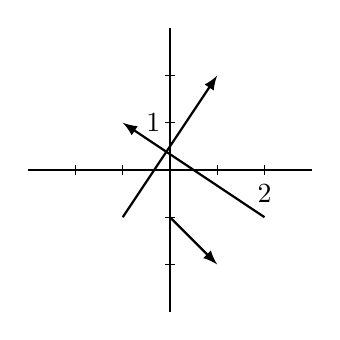
\begin{tikzpicture}[>=latex,scale=.6]
% Draw grid
\draw (-3,0)--(3,0);
\draw (0,-3)--(0,3);
\foreach \x in {-2,...,2}
 {\draw (\x,-.1)--(\x,.1);
  \draw (-.1,\x)--(.1,\x);
 };
\node[below] at (2,-0.1) {2};
\node[left] at (0,1) {1};
%Draw arrows
\draw [->,thick] (0,-1)--(1,-2) node [below right] {\vx};
\draw [->,thick] (-1,-1) -- (1,2) node [above right] {\vy};
\draw [->,thick] (2,-1) -- (-1,1) node [above left] {\vz};
\end{tikzpicture}
\end{center}
\mycaption{Drawing vectors $\protect\vx$, $\protect\vy$ and $\protect\vz$ in Example \ref{ex_draw_vectors_1}}
\label{fig:xyz}
\end{myfigure}
%\eexset
\vskip -2\baselineskip}\\

How does one draw the zero vector, $\zero =\bmx{c}0\\0\emx$?\footnote{Vectors are just special types of matrices. The zero vector, \zero, is a special type of zero matrix, \tto. It helps to distinguish the two by using different notation.} Following our basic procedure, we start by going 0 units in the $x$ direction, followed by 0 units in the $y$ direction. In other words, we don't go anywhere. 
In general, we don't actually draw \zero. At best, one can draw a dark circle at the origin to convey the idea that \zero, when starting at the origin, points to the origin.

In section \ref{sec:matrix_arithmetic_1} we learned about matrix arithmetic operations: matrix addition and scalar multiplication. Let's investigate how we can ``draw'' these operations.\\
\clearpage

\noindent \large \textsf{\textbf{ Vector Addition}} \normalsize\\

Given two vectors \vx\ and \vy, how do we draw the vector $\vx+\vy$? Let's look at this in the context of an example, then study the result.\\

%\enlargethispage{2\baselineskip}

\example{ex_add_vectors_1}{Let $$\vx = \bmx{c}1\\1\emx \quad \text{ and } \quad \vy = \bmx{c}3\\1\emx.$$ Sketch \vx, \vy\  and $\vx+\vy$.}
{A starting point for drawing each vector was not given; by default, we'll start at the origin. (This is in many ways nice; this means that the \textit{vector} $\bmx{c}3\\1\emx$ ``points'' to the \textit{point} (3,1).) We first compute $\vx+\vy$:
$$\vx+\vy = \bmx{c}1\\1\emx + \bmx{c}3\\1\emx = \bmx{c}4\\2\emx$$
Sketching each gives the picture in Figure \ref{fig:addvectors1}.
 %\eexset

\begin{myfigure}%[h!]
\btz[>=latex,scale=.75]
% Draw grid
\draw (-1,0)--(5,0);
\draw (0,-1)--(0,3);
\foreach \x in {1,...,4}
  \draw (\x,-.1)--(\x,.1);
\foreach \x in {1,...,2}
  \draw (-.1,\x)--(.1,\x);
\node[below] at (1,-0.1) {1};
\node[left] at (0,1) {1};
 
\draw[->,thick] (0,0)--(1,1) node [above] {\vx};
\draw[->,thick] (0,0)--(3,1) node [below right] {\vy};
\draw[->,thick] (0,0)--(4,2) node [above right] {$\vx+\vy$};


\etz
\mycaption{Adding vectors $\protect\vx$ and $\protect\vy$ in Example \ref{ex_add_vectors_1}}
\label{fig:addvectors1}
\end{myfigure}
\vskip -2\baselineskip}\\

This example is pretty basic; we were given two vectors, told to add them together, then sketch all three vectors. Our job now is to go back and try to see a relationship between the drawings of \vx, \vy\ and $\vx+\vy$. Do you see any?

Here is one way of interpreting the adding of \vx\ to \vy. Regardless of where we start, we draw \vx. Now, from the tip of \vx, draw \vy. The vector $\vx+\vy$ is the vector found by drawing an arrow from the \textit{origin} of \vx\ to the \textit{tip} of \vy.  Likewise, we could start by drawing \vy. Then, starting from the tip of \vy, we can draw \vx. Finally, draw $\vx+\vy$ by drawing the vector that starts at the origin of \vy\ and ends at the tip of \vx. 

The picture in Figure \ref{fig:addvectors2} illustrates this. The gray vectors demonstrate drawing the second vector from the tip of the first; we draw the vector $\vx+\vy$ dashed to set it apart from the rest. We also lightly filled the \textit{parallelogram} whose opposing sides are the vectors \vx\ and \vy. This highlights what is known as the \textit{Parallelogram Law}\index{Parallelogram Law}.

\enlargethispage{2\baselineskip}

\begin{myfigure}%[h!]
\btz[>=latex]
% Draw grid
\draw (-1,0)--(5,0);
\draw (0,-.5)--(0,2.5);
\foreach \x in {1,...,4}
  \draw (\x,-.1)--(\x,.1);
\foreach \x in {1,...,2}
  \draw (-.1,\x)--(.1,\x);
\node[below] at (1,-0.1) {1};
\node[left] at (0,1) {1};
 
\ifthenelse{\boolean{in_color}}{\fill[color=blue!10] (0,0)--(1,1)--(4,2)--(3,1)--(0,0);}
{\fill[color=black!5] (0,0)--(1,1)--(4,2)--(3,1)--(0,0); }
 
\draw[->,thick] (0,0)--(1,1) node [pos=.5,above] {\vx};
\draw[->,thick] (0,0)--(3,1) node [pos=.5,below] {\vy};
\draw[->,thick,gray] (3,1)--(4,2) node [pos=.5,below,black] {\vx};
\draw[->,thick,gray] (1,1)--(4,2) node [pos=.5,above,black] {\vy};
\draw[->,thick,dashed] (0,0)--(4,2) node [above right, black] {$\vx+\vy$};

\etz
\mycaption{Adding vectors graphically using the Parallelogram Law}
\label{fig:addvectors2}
\end{myfigure}

\keyidea{idea:Parallelogram}{\textbf{Parallelogram Law}\\

To draw the vector $\vx+\vy$, one can draw the parallelogram with \vx\ and \vy\ as its sides. The vector that points from the vertex where \vx\ and \vy\ originate to the vertex where \vx\ and \vy\ meet is the vector $\vx+\vy$.}


Knowing all of this allows us to draw the sum of two vectors without knowing specifically what the vectors are, as we demonstrate in the following example.\\

\example{ex_draw_add}{Consider the vectors \vx\ and \vy\ as drawn in Figure \ref{fig:draw_add_1}. Sketch the vector $\vx+\vy$.}
{
\begin{myfigure}%[h!]
\btz[>=latex,scale=.75]
\draw (-3,0)--(2.5,0);
\draw (0,-.5)--(0,2);

\draw[->, thick] (0,0)--(1,1) node[right] {\vx};
\draw[->, thick] (0,0)--(-2,1) node[above] {\vy};
\etz
\mycaption{Vectors $\protect\vx$ and $\protect\vy$ in Example \ref{ex_draw_add}}
\label{fig:draw_add_1}
\end{myfigure}%

%\enlargethispage{2\baselineskip}
We'll apply the Parallelogram Law, as given in Key Idea \ref{idea:Parallelogram}. As before, we draw $\vx+\vy$ dashed to set it apart. The result is given in Figure \ref{fig:draw_add_2}.

\begin{myfigure}%[h!]
\btz[>=latex,scale=.75]
\draw (-3,0)--(2.5,0);
\draw (0,-.5)--(0,2);

\draw[->, thick] (0,0)--(1,1) node[right] {\vx};
\draw[->, thick] (0,0)--(-2,1) node[above] {\vy};
\draw[->, thick, gray] (-2,1)--(-1,2) ;
\draw[->, thick, gray] (1,1)--(-1,2) ;
\draw[->,thick, dashed] (0,0)--(-1,2) node[above, black]{$\vx+\vy$};
\etz
\mycaption{Vectors $\protect\vx$, $\protect\vy$ and $\protect \vx+\protect\vy$ in Example \ref{ex_draw_add}}
\label{fig:draw_add_2}
\end{myfigure}%
%\vskip -3\baselineskip
}\clearpage
%\\

%\enlargethispage{-2\baselineskip}

\noindent \large \textsf{\textbf{ Scalar Multiplication}} \normalsize\\

After learning about matrix addition, we learned about scalar multiplication. We apply that concept now to vectors and see how this is represented graphically.\\

\example{ex_scalar_vect_1}{Let $$\vx = \bmx{c}1\\1\emx \quad \text{ and } \quad \vy = \bmx{c}-2\\1\emx.$$ Sketch \vx, \vy, 3\vx\ and $-1\vy$.}
{We begin by computing 3\vx\ and $-\vy$:$$ 3\vx = \bmx{c}3\\3\emx \quad \text { and } \quad -\vy = \bmx{c} 2\\-1\emx.$$

All four vectors are sketched in Figure \ref{fig:scalar_1}.

\begin{myfigure}%[h!]
\btz[>=latex,scale=.75]
% Draw grid
\draw (-3,0)--(4,0);
\draw (0,-2)--(0,4);
% label x
\foreach \x in {-2,...,3}
  \draw (\x,-.1)--(\x,.1);
% label y
\foreach \y in {-1,...,3}
  \draw (-.1,\y)--(.1,\y);
% label scale
\node[below] at (1,-0.1) {1};
\node[left] at (0,1) {1};

\draw[->, thick] (0,0)--(3,3) node[left] {3\vx};
\draw[->, thick] (0,0)--(1,1) node[left] {\vx};
\draw[->, thick] (0,0)--(-2,1) node[above] {\vy};
\draw[->, thick] (0,0)--(2,-1) node[above] {$-\vy$};

\etz
\mycaption{Vectors $\protect \vx$, $\protect \vy$, $3\protect \vx$ and $-\protect \vy$ in Example \ref{ex_scalar_vect_1}}
\label{fig:scalar_1}
\end{myfigure}%
\vskip -2\baselineskip}\\ %\eexset

As we often do, let us look at the previous example and see what we can learn from it. We can see that \vx\ and 3\vx\ point in the same direction (they lie on the same line), but 3\vx\ is just longer than \vx. (In fact, it looks like 3\vx\ is \textit{3} times longer than \vx. Is it? How do we measure length?)
 
 We also see that \vy\ and $-\vy$ seem to have the same length and lie on the same line, but point in the opposite direction. 
 
 A vector inherently conveys two pieces of information: length and direction. Multiplying a vector by a positive scalar $c$ stretches the vectors by a factor of $c$; multiplying by a negative scalar $c$ both stretches the vector and makes it point in the opposite direction. 
 
%\enlargethispage{3\baselineskip} 
 
 Knowing this, we can sketch scalar multiples of vectors without knowing specifically what they are, as we do in the following example.\\
 
\example{ex_draw_scale_1}{Let vectors \vx\ and \vy\ be as in Figure \ref{fig:draw_scale_1}. Draw 3\vx, $-2\vx$, and $\frac12\vy$.

\begin{myfigure}%[h!]
\btz[>=latex]
\draw (-3,0)--(3.5,0);
\draw (0,-.5)--(0,1.5);

\draw[->, thick] (0,0)--(1,.5) node[right] {\vx};
\draw[->, thick] (0,0)--(-2,1) node[above] {\vy};
\etz
\mycaption{Vectors $\protect\vx$ and $\protect\vy$ in Example \ref{ex_draw_scale_1}}
\label{fig:draw_scale_1}
\end{myfigure}%
}
{To draw 3\vx, we draw a vector in the same direction as \vx, but 3 times as long. To draw $-2\vx$, we draw a vector twice as long as \vx\ in the opposite direction; to draw $\frac12\vy$, we draw a vector half the length of \vy\ in the same direction as \vy. We again use the default of drawing all the vectors starting at the origin. All of this is shown in Figure \ref{fig:draw_scale_2}.

\begin{myfigure}%[h!]

\btz[>=latex]
\draw (-3,0)--(3.5,0);
\draw (0,-1.5)--(0,2);

\draw[->, thick] (0,0)--(1,.5) node[below] {\vx};
\draw[->, thick] (0,0)--(-2,1) node[above] {\vy};
\draw[->, thick] (0,0)--(3,1.5) node[right] {3\vx};
\draw[->, thick] (0,0)--(-2,-1) node[right] {$-2\vx$};
\draw[->, thick] (0,0)--(-1,.5) node[above=.1cm] {$\frac12\vy$};
\etz

\mycaption{Vectors $\protect\vx$, $\protect\vy$, $\protect 3\vx$, $\protect -2x$ and $\protect \frac12\vx$ in Example \ref{ex_draw_scale_1}}
\label{fig:draw_scale_2}
\end{myfigure}%
\vskip -2\baselineskip}\\   %\eexset

\noindent \large \textsf{\textbf{Vector Subtraction}} \normalsize \\

The final basic operation to consider between two vectors is that of vector subtraction: given vectors \vx\ and \vy, how do we draw $\vx-\vy$?

If we know explicitly what \vx\ and \vy\ are, we can simply compute what $\vx-\vy$ is and then draw it. We can also think in terms of vector addition and scalar multiplication: we can \textit{add} the vectors $\vx + (-1)\vy$. That is, we can draw \vx\ and draw $-\vy$, then add them as we did in Example \ref{ex_draw_add}. This is especially useful we don't know explicitly what \vx\ and \vy\ are.\\

\example{ex_subtract}{Let vectors \vx\ and \vy\ be as in Figure \ref{fig:subtract_1}. Draw $\vx-\vy$.

\begin{myfigure}%[h!]
\btz[>=latex]
\draw (-3,0)--(3.5,0);
\draw (0,-.5)--(0,1.5);

\draw[->, thick] (0,0)--(1,.5) node[below] {\vx};
\draw[->, thick] (0,0)--(-1,1) node[above] {\vy};

\etz
\mycaption{Vectors $\protect\vx$ and $\protect\vy$ in Example \ref{ex_subtract}}
\label{fig:subtract_1}
\end{myfigure}%
}
{To draw $\vx-\vy$, we will first draw $-\vy$ and then apply the Parallelogram Law to add \vx\ to $-\vy$. See Figure \ref{fig:subtract_2}.

\begin{myfigure}%[h!]
\btz[>=latex]
\draw (-3,0)--(3.5,0);
\draw (0,-1.5)--(0,2);

\draw[->, thick] (0,0)--(1,.5) node[below] {\vx};
\draw[->, thick] (0,0)--(-1,1) node[above] {\vy};
\draw[->, thick] (0,0)--(1,-1) node[below] {$-\vy$};
\draw[->, thick, gray] (1,-1)--(2,-.5) ;
\draw[->, thick, gray] (1,.5)--(2,-.5) ;
\draw[->, thick, dashed] (0,0)--(2,-.5) node[right,black] {$\vx-\vy$};

\etz
\mycaption{Vectors $\protect\vx$, $\protect\vy$ and $\protect \vx - \protect \vy$ in Example \ref{ex_subtract}}
\label{fig:subtract_2}
\end{myfigure}%
\vskip -2\baselineskip}\\

In Figure \ref{fig:subtract_3}, we redraw Figure \ref{fig:subtract_2} from Example \ref{ex_subtract} but remove the gray vectors that tend to add clutter, and we redraw the vector $\vx-\vy$ dotted so that it starts from the tip of \vy.\footnote{Remember that we can draw vectors starting from anywhere.} Note that the dotted version of $\vx-\vy$ points from \vy\ to \vx. This is a ``shortcut'' to drawing $\vx-\vy$; simply draw the vector that starts at the tip of \vy\ and ends at the tip of \vx. This is important so we make it a Key Idea.

\begin{myfigure}%[h!]
\btz[>=latex]
\draw (-3,0)--(3.5,0);
\draw (0,-1.25)--(0,1.5);

\draw[->, thick] (0,0)--(1,.5) node[right] {\vx};
\draw[->, thick] (0,0)--(-1,1) node[above] {\vy};
\draw[->, thick] (0,0)--(1,-1) node[below] {-\vy};
\draw[->, thick, dotted] (-1,1)--(1,.5) node[above,pos=.8,black] {$\vx-\vy$};
\draw[->, thick, dashed] (0,0)--(2,-.5) node[right,black] {$\vx-\vy$};

\etz
\mycaption{Redrawing vector $\protect\vx - \protect\vy$}
\label{fig:subtract_3}
\end{myfigure}%

\keyidea{idea:vector_subtract}{\textbf{Vector Subtraction}\\

To draw the vector $\vx-\vy$, draw \vx\ and \vy\ so that they have the same origin. The vector $\vx-\vy$ is the vector that starts from the tip of \vy\ and points to the tip of \vx.}


Let's practice this once more with a quick example.\\
\enlargethispage{2\baselineskip}
%\clearpage

\example{ex_subtract_quick}{Let \vx\ and \vy\ be as in Figure \ref{fig:subtract_quick_1} (a). Draw $\vx-\vy$.
%
%\begin{myfigure}%[h!]
%\btz[>=latex,scale=.6]
%\draw (-.5,0)--(1.5,0);
%\draw (0,-1.5)--(0,1.5);
%
%\draw[->, thick] (0,0)--(1,1) node[above] {\vy};
%\draw[->, thick] (0,0)--(1,-1) node[below] {\vx};
%\etz
%\mycaption{Vectors $\protect\vx$ and  $\protect\vy$ in Example \ref{ex_subtract_quick}}
%\label{fig:subtract_quick_1}
%\end{myfigure}%
}
{We simply apply Key Idea \ref{idea:vector_subtract}: we draw an arrow from \vy\ to \vx. We do so in Figure \ref{fig:subtract_quick_2}; $\vx-\vy$ is dashed.

\begin{myfigure}%[h!]
\btz[>=latex,scale=.75]
\begin{scope}
\draw (-.5,0)--(1.5,0);
\draw (0,-1.5)--(0,1.5);

\draw[->, thick] (0,0)--(1,1) node[above] {\vy};
\draw[->, thick] (0,0)--(1,-1) node[below] {\vx};
\draw (0.5,-2) node [below] {(a)};
\end{scope}
\begin{scope}[shift={(5,0)}]
\draw (-.5,0)--(1.5,0);
\draw (0,-1.5)--(0,1.5);

\draw[->, thick] (0,0)--(1,1) node[above] {\vy};
\draw[->, thick] (0,0)--(1,-1) node[below] {\vx};
\draw[->, thick, dashed] (1,1)--(1,-1) node[pos=.8,right,black] {$\vx-\vy$} ;
\draw (0.5,-2) node [below] {(b)};
\end{scope}
\etz
\mycaption{Vectors $\protect\vx$, $\protect\vy$ and $\protect\vx - \protect \vy$ in Example \ref{ex_subtract_quick}}
\label{fig:subtract_quick_2}
\end{myfigure}%
\vskip -2\baselineskip
}\\ %\eexset

%\pagebreak



\noindent \large \textsf{\textbf{Vector Length}} \normalsize\\

When we discussed scalar multiplication, we made reference to a fundamental question: How do we measure the length of a vector? Basic geometry gives us an answer in the two dimensional case that we are dealing with right now, and later we can extend these ideas to higher dimensions.

Consider Figure \ref{fig:vector_length}. A vector \vx\ is drawn in black, and dashed and dotted lines have been drawn to make it the hypotenuse of a right triangle.

\begin{myfigure}%[h!]
\btz[>=latex,scale=.5]
% Draw grid
\draw (-1,0)--(5,0);
\draw (0,-1)--(0,5);
\foreach \x in {1,...,4}
  \draw (\x,-.1)--(\x,.1);
\foreach \x in {1,...,4}
  \draw (-.1,\x)--(.1,\x);
\node[below] at (1,-0.1) {1};
\node[left] at (0,1) {1};
 
\draw[dashed,thick] (0,1)--(4,1);
\draw[thick,dotted] (4,1)--(4,4);
\draw[->,thick] (0,1)--(4,4) node [above] {\vx};

\etz
\mycaption{Measuring the length of a vector}
\label{fig:vector_length}
\end{myfigure}%

It is easy to see that the dashed line has length 4 and the dotted line has length 3. We'll let $c$ denote the length of \vx; according to the Pythagorean Theorem, $4^2+3^2 = c^2$. Thus $c^2 = 25$ and we quickly deduce that $c=5$. 

Notice that in our figure, \vx\ goes to the right 4 units and then up 3 units. In other words, we can write $$\vx = \bmx{c} 4\\3\emx.$$ We learned above that the length of \vx\ is $\sqrt{4^2+3^2}$.\footnote{Remember that $\sqrt{4^2+3^2} \neq 4+3$!} This hints at a basic calculation that works for all vectors \vx, and we define the length of a vector according to this rule.

\definition{def:vector_length}{\textbf{Vector Length}\index{vector!length}\\

Let $$\vx = \bmx{c}x_1\\x_2\emx.$$ The \textit{length} of \vx, denoted $||\vx||$, is $$||\vx|| = \sqrt{x_1^2+x_2^2}.$$}

\example{ex_length}{Find the length of each of the vectors given below.
$$ \vx[1] = \bmx{c}1\\1\emx \quad \vx[2] = \bmx{c} 2\\-3\emx \quad \vx[3]=\bmx{c} .6\\.8 \emx \quad \vx[4]=\bmx{c} 3\\0\emx$$}
{We apply Definition \ref{def:vector_length} to each vector.\\

\begin{align*}
||\vx[1]|| &= \sqrt{1^2+1^2} = \sqrt{2}.\\
||\vx[2]|| &= \sqrt{2^2+(-3)^2} = \sqrt{13}.\\
||\vx[3]|| &= \sqrt{.6^2 +.8^2} = \sqrt{.36+.64} = 1.\\
||\vx[4]|| &= \sqrt{3^2+0} = 3.
\end{align*}
\vskip -1\baselineskip
}\\ % \eexset
 

Now that we know how to compute the length of a vector, let's revisit a statement we made as we explored Examples \ref{ex_scalar_vect_1} and \ref{ex_draw_scale_1}: ``Multiplying a vector by a positive scalar $c$ stretches the vectors by a factor of $c$ $\ldots$'' At that time, we did not know how to measure the length of a vector, so our statement was unfounded. In the following example, we will confirm the truth of our previous statement.\\

\example{ex_scalar_vect_2}{Let $\vx = \bmx{c} 2\\-1\emx$. Compute $||\vx||$, $||3\vx||$, $||-2\vx||$, and $||c\vx||$, where $c$ is a scalar.}
{We apply Definition \ref{def:vector_length} to each of the vectors.\\

$||\vx|| = \sqrt{4+1} = \sqrt{5}$.

Before computing the length of $||3\vx||$, we note that $3\vx = \bmx{c} 6\\-3\emx$.\\

$||3\vx|| = \sqrt{36+9} = \sqrt{45} = 3\sqrt{5} = 3||\vx||.$

Before computing the length of $||-2\vx||$, we note that $-2\vx = \bmx{c} -4\\2\emx$.\\

$||-2\vx|| = \sqrt{16+4} = \sqrt{20} = 2\sqrt{5} = 2||\vx||.$

Finally, to compute $||c\vx||$, we note that $c\vx = \bmx{c} 2c\\-c\emx$. Thus:\\

$||c\vx|| = \sqrt{(2c)^2 + (-c)^2} = \sqrt{4c^2 + c^2} = \sqrt{5c^2} = |c|\sqrt{5}.$\\

This last line is true because the square root of any number squared is the \textit{absolute value} of that number (for example, $\sqrt{(-3)^2} = 3$).}\\% \eexset

The last computation of our example is the most important one. It shows that, in general, multiplying a vector \vx\ by a scalar $c$ stretches \vx\ by a factor of $|c|$ (and the direction will change if $c$ is negative). This is important so we'll make it a Theorem.

\theorem{thm:vect_length}{\textbf{Vector Length and Scalar Multiplication}\\

Let \vx\ be a vector and let $c$ be a scalar. Then the length of $c\vx$ is $$||c\vx|| = |c|\cdot ||\vx||.$$}

\noindent \large \textsf{\textbf{Matrix $-$ Vector Multiplication}} \normalsize\\

The last arithmetic operation to consider visualizing is matrix multiplication. Specifically, we want to visualize the result of multiplying a vector by a matrix. In order to multiply a 2D vector by a matrix and get a 2D vector back, our matrix must be a square, $2\times 2$ matrix.\footnote{We can multiply a $3\times 2$ matrix by a 2D vector and get a 3D vector back, and this gives very interesting results. See section \ref{sec:lin_trans}.}

We'll start with an example. Given a matrix \tta\ and several vectors, we'll graph the vectors before and after they've been multiplied by \tta\ and see what we learn.\\

\example{ex_mv_1}{Let \tta\ be a matrix, and \vx, \vy, and \vz\ be vectors as given below.
$$\tta = \bmx{cc} 1&4\\2&3\emx,  \quad \vx = \bmx{c} 1\\1\emx, \quad \vy = \bmx{c}-1\\1\emx, \quad \vz = \bmx{c} 3\\-1\emx$$
Graph \vx, \vy\ and \vz, as well as \tta\vx, \tta\vy\ and \tta\vz.}
{\begin{myfigure}%[h!]
\begin{center}
\begin{tikzpicture}[x={(.6cm,0)},y={(0,.6cm)}, >=latex]

\drawxlines{-2.5}{6.5}{-2,...,6};
\drawylines{-1.5}{5.5}{-1,...,5};
\draw [->] (0,0)--(1,1) node [right ] {\vx};
\draw [->] (0,0)--(-1,1) node [above] {\vy};
\draw [->] (0,0)--(3,-1) node [below right] {\vz};
\draw [->] (0,0)--(5,5) node [above right] {\tta\vx};
\draw [->] (0,0)--(3,1) node [right] {\tta\vy};
\draw [->] (0,0)--(-1,3) node [above] {\tta\vz};

\end{tikzpicture}
\end{center}
\mycaption{Multiplying vectors by a matrix in Example \ref{ex_mv_1}.}
\label{fig:mv_1}
\end{myfigure}%

It is straightforward to compute: $$\tta\vx = \bmx{c} 5\\5\emx,\quad \tta\vy = \bmx{c} 3\\1\emx, \quad \text{ and } \quad \tta\vz = \bmx{c} -1\\3\emx.$$ The vectors are sketched in Figure \ref{fig:mv_1}
}\\  %\eexset

There are several things to notice. When each vector is multiplied by \tta, the result is a vector with a different length (in this example, always longer), and in two of the cases (for \vy\ and \vz), the resulting vector points in a different direction. 

This isn't surprising. In the previous section we learned about matrix multiplication, which is a strange and seemingly unpredictable operation. Would you expect to see some sort of immediately recognizable pattern appear from multiplying a matrix and a vector?\footnote{This is a rhetorical question; the expected answer is ``No.''} In fact, the surprising thing from the example is that \vx\ and \tta\vx\ point in the same direction! Why does the direction of \vx\ not change after multiplication by \tta? (We'll answer this in Section \ref{sec:eigen} when we learn about something called ``eigenvectors.'')

%One may recall that \tta\ and \vx\ previously appeared in Section \ref{sec:eigen}, where \vx\ is an eigenvector of \tta\ with an \el\ of 5. Therefore this example lets us visualize the significance of \ev s: ``normally,'' when a vector is multiplied by a matrix, its length and direction changes. However, when the vector is an \ev, its direction does not change, only its length\footnote{If the \el\ is 1, then of course, nothing changes. The careful reader will also note that if the $\el <0$, then the resulting vector will point in the opposite direction, meaning the direction \textit{did} change. However, in this case, \vx\ and \tta\vx\ lie on the same line which is still significant}.

Different matrices act on vectors in different ways.\footnote{That's one reason we call them ``different.''} Some always increase the length of a vector through  multiplication, others always decrease the length, others increase the length of some vectors and decrease the length of others, and others still don't change the length at all. A similar statement can be made about how matrices affect the direction of vectors through multiplication: some change every vector's direction, some change ``most'' vector's direction but leave some the same, and others still don't change the direction of any vector.

How do we set about studying how matrix multiplication affects vectors? We could just create lots of different matrices and lots of different vectors, multiply, then graph, but this would be a lot of work with very little useful result. It would be too hard to find a pattern of behavior in this.\footnote{Remember, that's what mathematicians do. We look for patterns.}

Instead, we'll begin by using a technique we've employed often in the past. We have a ``new'' operation; let's explore how it behaves with ``old'' operations. Specifically, we know how to sketch vector addition. What happens when we throw matrix multiplication into the mix? Let's try an example.\\

\example{ex_mv_2}{Let \tta\ be a matrix and \vx\ and \vy\ be vectors as given below. $$\tta = \bmx{cc} 1 & 1\\1&2\emx, \quad \vx = \bmx{c} 2\\1\emx, \quad \vy = \bmx{c} -1\\1\emx$$
Sketch $\vx+\vy$, \tta\vx, \tta\vy, and $\tta(\vx+\vy)$. }
{It is pretty straightforward to compute: 
$$\vx+\vy = \bmx{c} 1\\2\emx;\quad \tta\vx = \bmx{c}3\\4\emx; \quad \tta\vy = \bmx{c} 0\\1\emx,\quad \tta(\vx+\vy) = \bmx{c} 3\\5\emx.$$

In Figure \ref{fig:mv_2}, we have graphed the above vectors and have included dashed gray vectors to highlight the additive nature of $\vx+\vy$ and $\tta(\vx+\vy)$. Does anything strike you as interesting?

\begin{myfigure}%[h!]
\begin{center}
\begin{tikzpicture}[x={(1cm,0)},y={(0,1cm)}, >=latex]
\drawxlines{-1}{4}{0,...,3};
\drawylines{-1}{5}{0,...,4};
\draw [->] (0,0)--(2,1) node [right] {\vx};
\draw [->] (0,0)--(-1,1) node [left ] {\vy};
\draw [->,gray,dashed] (2,1) -- (1,2);
\draw [->] (0,0)--(1,2) node [above] {$\vx+\vy$};
\draw [->] (0,0)--(3,4) node [above right] {\tta\vx};
\draw [->] (0,0)--(0,1) node [above left] {\tta\vy};
\draw [->,gray,dashed] (3,4) -- (3,5);
\draw [->] (0,0)--(3,5) node [above] {$\tta(\vx+\vy)$};
\end{tikzpicture}
\end{center}
\mycaption{Vector addition and matrix multiplication in Example \ref{ex_mv_2}.}
\label{fig:mv_2}
\end{myfigure}%

Let's not focus on things which don't matter right now: let's not focus on how long certain vectors became, nor necessarily how their direction changed. Rather, think about how matrix multiplication interacted with the vector addition.

In some sense, we started with three vectors, \vx, \vy, and $\vx+\vy$. This last vector is special; it is the sum of the previous two. Now, multiply all three by \tta. What happens? We get three new vectors, but the significant thing is this: the last vector is still the sum of the previous two! (We emphasize this by drawing dotted vectors to represent part of the Parallelogram Law.)

Of course, we knew this already: we already knew that $\tta\vx + \tta\vy = \tta(\vx+\vy)$, for this is just the Distributive Property. However, now we get to see this graphically.}\\ %\eexset

In Section \ref{sec:geom_3} we'll study in greater depth how matrix multiplication affects vectors and the whole Cartesian plane. For now, we'll settle for simple practice: given a matrix and some vectors, we'll multiply and graph. Let's do one more example.\\


\example{ex_mv_23}{Let \tta, \vx, \vy, and \vz\ be as given below.
$$\tta = \bmx{cc} 1&-1\\1&-1\emx,  \quad \vx = \bmx{c} 1\\1\emx, \quad \vy = \bmx{c}-1\\1\emx, \quad \vz = \bmx{c} 4\\1\emx$$
Graph \vx, \vy\ and \vz, as well as \tta\vx, \tta\vy\ and \tta\vz.}
{\begin{myfigure}%[h!]
\begin{center}
\begin{tikzpicture}[x={(.6cm,0)},y={(0,.6cm)}, >=latex]

\drawxlines{-2.5}{3.5}{-2,...,3};
\drawylines{-2.5}{3.5}{-2,...,3};
\draw [->] (0,0)--(1,1) node [right ] {\vx};
\draw [->] (0,0)--(-1,1) node [above] {\vy};
\draw [->] (0,0)--(4,1) node [above] {\vz};
\draw (0,0) node [below right] {\tta\vx};
\draw [->] (0,0)--(-2,-2) node [below left] {\tta\vy};
\draw [->] (0,0)--(3,3) node [above] {\tta\vz};

\end{tikzpicture}
\end{center}
\mycaption{Multiplying vectors by a matrix in Example \ref{ex_mv_23}.}
\label{fig:mv_23}
\end{myfigure}%

It is straightforward to compute: $$\tta\vx = \bmx{c} 0\\0\emx,\quad \tta\vy = \bmx{c} -2\\-2\emx, \quad \text{ and } \quad \tta\vz = \bmx{c} 3\\3\emx.$$ The vectors are sketched in Figure \ref{fig:mv_23}.

These results are interesting. While we won't explore them in great detail here, notice how \vx\ got sent to the zero vector. Notice also that \tta\vx, \tta\vy\ and \tta\vz\ are all in a line (as well as \vx!). Why is that? Are \vx, \vy\ and \vz\ just special vectors, or would any other vector get sent to the same line when multiplied by \tta?\footnote{Don't just sit there, try it out!}
}\\

%%%%%%%%%%%%%%%%%%%
%%%%%%%%%%%%%%%%%%%

This section has focused on vectors in two dimensions. Later on in this book, we'll extend these ideas into three dimensions (3D). 
%
%So far we've learned how to add matrices together and how to multiply a matrix by a scalar. In the next section we'll  consider what it means to multiply two matrices together.\\

In the next section we'll take a new idea (matrix multiplication) and apply it to an old idea (solving systems of linear equations). This will allow us to view an old idea in a new way -- and we'll even get to ``visualize'' it.\\

\clearpage

\printexercises{exercises/05_01_exercises} 
 
 
%%
% Given the idea of length, measure the length of \vx and 3\vx
% Section 5.2 - extend into 3D
% Section 5.3 - investigate matrix-vector multiplication

% Exercise Ideas
% Given explicit vectors, draw, scale, add, subtract
% Given drawn vectors, do the same as above
% Give length of vectors \vx, 5\vx, -2\vx, -\vx explicitly